% !Mode:: "TeX:UTF-8"
%\chapter{车联网技术的网络资源优化理论基础}
\chapter{基于博弈论的鲁棒干扰管理异构车载网络中的大规模空地一体化通信
异构车载网络}

\begin{comment}
\label{chap:figures}

插图主要涉及到:单个居中图形;两个并排图形;两个以上的并排或者堆叠的图形;图题;图形的引用;
\end{comment}
\section{引言}\label{section2-1}
作为智能交通系统(ITS)最有前途的解决方案,车联网(IoV)有望满足快速增长的需求,如交通效率、驾驶体验和事故处理。然而,由于车辆密度和用户需求的快速增加,单小区网络的频谱效率较低
\cite{TFL}。因此,异构车载网络的部署已成为一种趋势。

近年来,空地一体化作为提高无线通信质量的最可行的解决方案之一,引起了工业界和学术界的广泛关注。由于部署灵活、远程操作和中继能力,选择空中无人机来辅助地面网络\cite{ACO}。然而,当无人机加入异构场景时,空地综合通信网络将面临两大挑战。首先,当使用信道复用模式来提高频谱效率时,多用户干扰是一个棘手的问题。有效和稳健的通信在很大程度上受到多用户干扰的影响,特别是在不确定的信道环境中,因此实现有效的干扰管理是一个重大挑战\cite{CCO}。其次,空地集成异构车辆网络(AGHVN)是分层的,其中蜂窝用户(CUE)和车辆用户(VUE)分别充当领导者和追随者。然而,CUE和VUE是不同的利益相关者,他们为自己的利益而竞争。平衡各方利益是一项挑战。因此,空地一体化异构车载网络的广泛部署仍然带来紧迫的挑战。
\begin{comment}
\subsection{NOMA技术的理论基础}\label{section2-1-1}
大多数情况下,需要插入的图形是单个的时候可以使用如下环境:

\subsection{CR技术的理论基础}\label{section2-1-2}
其中的参数“[width=$\backslash$textwidth]”指定图形的宽度0.6倍页宽。最后的效果如图\ref{ysulogo}所示。
\begin{figure}[hptb!]
 \centering\small
 
\includegraphics[width=0.6\textwidth]{ysulogo}
 \Figcaption{单个居中图形}\label{ysulogo}
\end{figure}
\subsection{MEC技术的理论基础}\label{section2-1-3}

最终结果如图\ref{fig-dbfig}所示。
\begin{figure}[hptb!]
  \centering\small
  \begin{minipage}[t]{0.5\linewidth}
    \centering
    \includegraphics[width=\textwidth]{chp-2_bessel_j}
    (a) 子图a图题子图a图题子图a图题
  \end{minipage}%
  \begin{minipage}[t]{0.5\textwidth}
    \centering
    \includegraphics[width=\textwidth]{chp-2_bessel_k}
    (b) 子图b图题子图b图题子图b图题
  \end{minipage}
    \Figcaption{两个并排图形}\label{fig-dbfig}
 \end{figure}
\end{comment}

\section{问题构建}\label{section2-2}
\subsection{系统及信道模型}\label{section2-2-1}
我们考虑了一种上行链路空地一体化通信场景,在这种场景中,众多车对无人机(V2U)小区覆盖在一个宏蜂窝之下。如图 1 所示,无人机固定悬停并部署在交通拥堵路段,负责接收其覆盖范围内车辆的信号并将其发送到基站(BS)。值得注意的是,所有无人机都是双工的,配备有接收天线和发射天线,因此接收和发射过程可以同时完成。通信中的CUE和VUE集合分别索引为$\mathcal{S}_0:= \{0\}$ 和$\mathcal{S}_l:=\{1, 2,..., N\}$ 。为了提高频谱利用率,实现多用户联合通信,V2U 通信重复使用了 CUE 的上行信道。但是会产生严重的多用户干扰,限制了信号链路的通信。如图 1 所示,信号链路(蜂窝链路和同信道 V2U 链路)和干扰链路(CUE-V 链路、V-BS 链路和 V2U 干扰链路)被区分开来。

假设无人飞行器的飞行高度为 $H_n$,则 VUE$_{k}$ 与 UAV$_{n}$ 之间的距离为:
\begin{eqnarray}\label{1}
h_{k,n}=\sqrt{H_n^2+(\|W_k-W_n\|)^2},           &k\in \mathcal{N}, n\in \mathcal{N}
\end{eqnarray}
其中 $W_k$ 和 $W_n$ 是 VUE$_{k}$ 与 UAV$_{n}$的位置信息,  CUE 与BS之间的距离为:
\begin{eqnarray}\label{2}
h_{0,0}=\sqrt{H_0^2+(\|W_0-W_{BS}\|)^2},
\end{eqnarray}
其中,$W_0$ 和 $W_{BS}$ 为 CUE 和 BS 的位置,$H_0$ 为 BS 上信号接收器的垂直高度。VUE$_{k}$ 与 BS 之间的距离为 $h_{k,0}$,CUE 与 UAV$_{n}$ 之间的距离为 $h_{0,n}$。$h_{k,0}$和$h_{0,n}$的表达式类似于(\ref{1})和(\ref{2})。
\begin{figure}[htbp]
\centerline{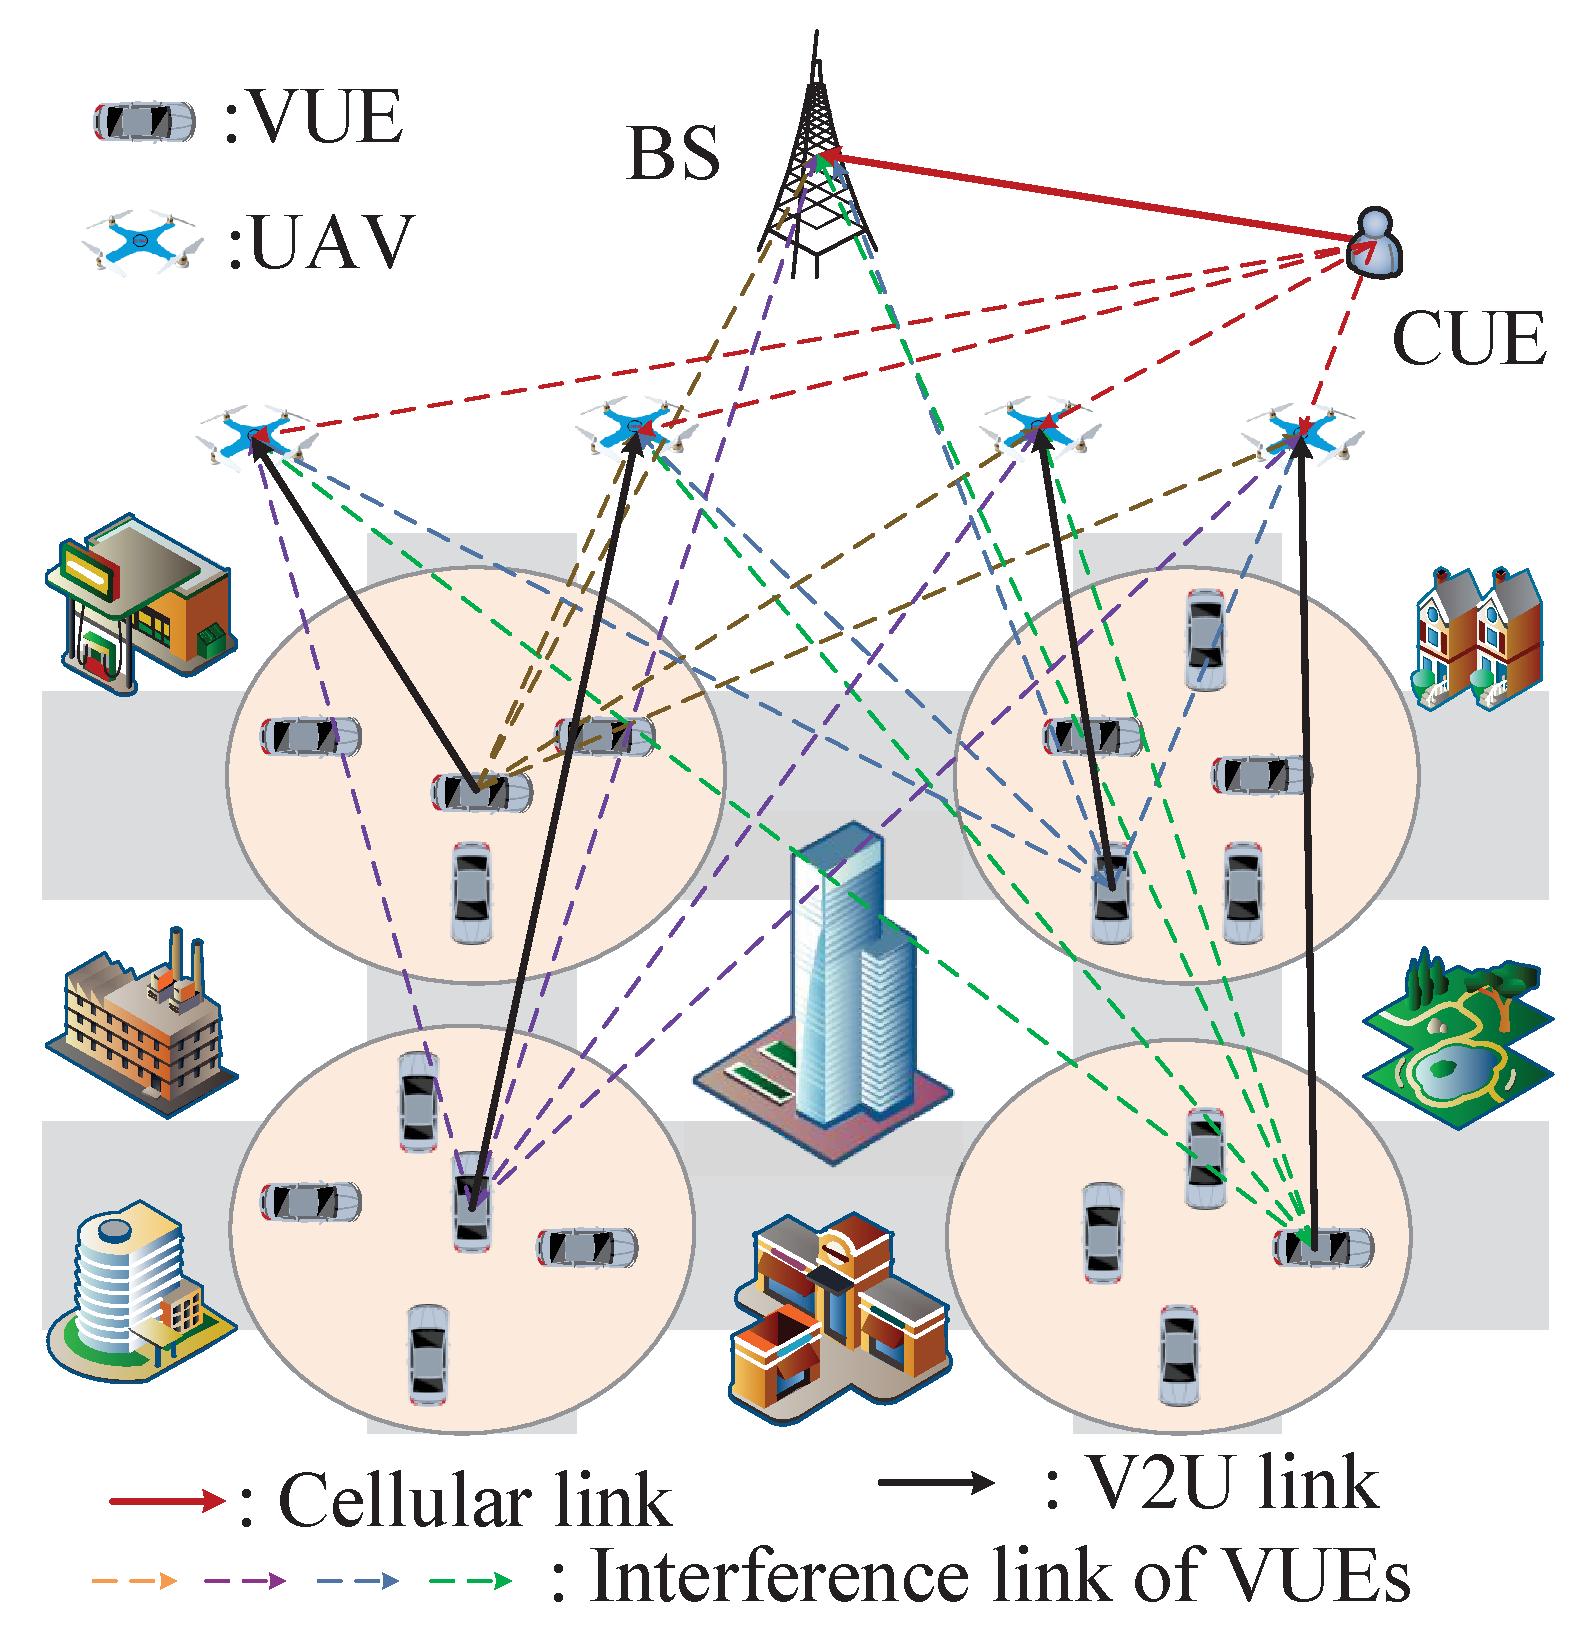
\includegraphics[width=8cm]{figures//chap2//1.eps}}
\center{\footnotesize Fig. 1 System model}
\end{figure}

蜂窝链路和同信道 V2U 链路的大规模衰落可分别表示为:
\begin{eqnarray}\label{3}
g_{0,0}=L_{0,0}h_{0,0}^{-\alpha},
\end{eqnarray}
\begin{eqnarray}\label{4}
g_{n,n}=L_{k,n}h_{k,n}^{-\alpha},          &k, n\in \mathcal{N}, k=n
\end{eqnarray}
其中,$L_{0,0}$ 和 $L_{n,n}$ 是蜂窝链路和同信道 V2U 链路的阴影衰减效应。$\alpha$ 是路径损耗指数。虽然车辆与无人机之间的传输链路可视为借助无人机在道路上空进行的 LoS 通信,但仍存在一些影响信道增益的因素,如通信终端的相对移动、信道估计误差以及不可避免的信道不确定性。因此,小尺度衰落不容忽视。根据 \cite{CCO},它遵循截断指数分布。为了描述信道增益的不确定性,引入了一个参数 $G$,$G$ 是一个独立的同分布随机变量,其概率密度函数为 $f_G (x)=e^{-x}$ 。
信号链路 $n$ 的实时信噪比(SINR)可表示为:
\begin{eqnarray}\label{5}
\gamma_{n}(p_n)=\frac{p_{n}G g_{n,n}}{I_n}, k\in\mathcal{N},n\in\mathcal{N},
\end{eqnarray}
其中,$g_{n,n}$ 是给定时隙内的估计增益。同信道 V2U 链路 $n$ 的干扰可视为测量值,其表达式为:
\begin{eqnarray}\label{6}
I_n=p_0 g_{0,n}+\!\!\!\sum\limits_{k=1,k\neq n}^N\!\!\!\! p_k g_{k,n}+\delta^2, \quad k\in\mathcal{N},n\in\mathcal{N},
\end{eqnarray}
其中,$p_k$ 表示第 k 个 VUE 的传输功率。$p_0$ 是 CUE 的传输功率。$\delta^2$ 是噪声干扰。

为处理不确定参数 $G$,确保 V2U 通信质量,我们引入了以下中断概率约束、
\begin{eqnarray}\label{7}
\textrm{Pr}\left\{\gamma_{n} \leq \gamma_{th}\right\}\geq1-\varepsilon,\quad  n\in\mathcal{N}
\end{eqnarray}
其中,$\gamma_{n}$ 表示第 n 个同频 V2U 链路的瞬时 SINR。$\gamma_{th}$是事先给定的阈值,代表目标 SINR。$varepsilon$ 是中断概率阈值,$\varepsilon \ in (0,1)$ 。

考虑了不确定的信道增益,并使用遍历容量来显示网络性能。
\begin{eqnarray}\label{8}
R_{er}=\int_{0}^{\infty} W \log(1+\gamma_{n})\Pr(\gamma_{n})\, d(\gamma_{n}),
\end{eqnarray}
其中,$W$ 是重用信道的带宽,$\Pr(\gamma_{n})$ 是 $\gamma_{n}$ 的概率分布函数。 根据詹森不等式
认为
\begin{eqnarray}\label{9}
 \begin{array}{lll}
&\!\!\!\!\!\!\mathbb{E}\{W \log(1+\gamma_{n}\}=\int_{0}^{\infty} W \log(1+\gamma_{n})\ \Pr(\gamma_{n})\, d(\gamma_{n})\\
&\quad\quad\quad\quad\quad\quad\quad\!\!<W\log(1+\mathbb{E}\{\gamma_{n}\})\\
&\quad\quad\quad\quad\quad\quad\quad\!\!=W\log(1+\bar{\gamma}_{n}),
 \end{array}
\end{eqnarray}
其中 $\bar{\gamma}_{n}\!=\mathbb{E}\{\!\frac{p_{n}G g_{n,n}}{I_n}\}
\!=\!\frac{p_{n}g_{n,n}}{I_n}$. 这也是香农容量是遍历容量的上限,通过信道编码技术可以使遍历容量接近上限。
因此,根据香农定理计算出的 VUE 的确定性等效传输速率为:
\begin{eqnarray}\label{10}
R_{n}=W\log(1+\bar{\gamma}_{n}(p_n)),\quad  n\in\mathcal{N}.
\end{eqnarray}

\subsection{博弈论问题}\label{section2-2-1}
在空地一体化异质车载网络(AGHVN)中,频谱所有者 CUE 可以对干扰进行定价,并将 VUE 的收费作为其利润。在 V2U 小区中,VUE 的效用是传输速率与购买干扰成本之间的差额。考虑到 CUE 和 VUE 都是自私自利的,它们都愿意为自己的利益而竞争。因此,数学框架自然符合 Stackelberg 博弈模型,其中 CUE 和 VUE 分别是领导者和追随者。此外,还考虑了 CUE 的通信约束。$n_{th}$ V2U 单元的下子博弈可表述为:
\begin{comment}
\begin{eqnarray}\label{11}
\begin{array}{rl}
&\!\!\!\!\!\!P_1: \max\limits_{p_{n}} U_{n}=R_{n}\!\!-c_{n} p_n g_{n,0}\\ [10pt]
s.t. &\left\{
\begin{array}{ll}
     \textrm{Pr}\left\{\gamma_{n}(p_n) \geq \gamma_{th}\right\}\geq1-\varepsilon\\
     0\leq p_n\leq p_{n,\textrm{max}} %\quad  \forall i\in\mathcal{I}, j\in\mathcal{J}
\end{array}
\right.
\end{array}
\end{eqnarray}
\end{comment}

\begin{align}
&P_1: \max\limits_{p_{n}} U_{n}=R_{n}\!\!-c_{n} p_n g_{n,0}                \label{E2-11}\\
\text { s.t. }
& \textrm{Pr}\left\{\gamma_{n}(p_n) \geq \gamma_{th}\right\}\geq1-\varepsilon           \tag{\ref{E2-11}{-1}}      \label{E2-11-1}\\  %信噪比中断概率约束
& 0\leq p_n\leq p_{n,\textrm{max}}                           \tag{\ref{E2-11}{-2}}      \label{E2-11-2}  %功率阈值
\end{align}
\section{博弈问题求解}\label{section2-3}
\subsection{概率约束的转化}\label{section2-3-1}
\subsection{求解下层子问题}\label{section2-3-2}
\subsection{求解上层子问题}\label{section2-3-3}
\section{仿真验证及性能分析}\label{section2-4}

\section{本章小结}\label{section2-5}
在章节中,我们提出了一种基于鲁棒博弈的资源分配算法,以实现AGHVN中的有效信息传输。在新的优化方案中,关注用户之间的博弈关系,制定实时功率分配和定价策略,以最大限度地提高用户的利益。具体来说,为了保证系统的鲁棒性,引入概率约束来保证用户服务的可靠性和稳定性。由于通道不确定性的存在,概率形式是非凸的且难以处理的,在凸优化过程中采用了指数积分方法。根据仿真结果,功率和价格在几个步骤内收敛到最优值。我们还可以得出结论,Stackelberg对策优化方案表现出更好的鲁棒性。因此,在具有复杂多用户干扰和信道不确定性的空地一体化异构车载通信场景下,所提出的基于鲁棒博弈的资源分配算法是有效的。


\begin{comment}
\begin{verbatim}
\begin{figure}[hptb!]
  \centering\small
  \begin{minipage}[t]{0.5\linewidth}
    \centering
    \includegraphics[width=\textwidth]{chp-2_bessel_j}
    (a) 子图a图题
  \end{minipage}%
  \begin{minipage}[t]{0.5\textwidth}
    \centering
    \includegraphics[width=\textwidth]{chp-2_bessel_k}
    (b) 子图b图题
  \end{minipage}  \\
  \begin{minipage}[t]{0.5\textwidth}
    \centering
    \includegraphics[width=\textwidth]{chp-2_bessel_i}
    (c) 子图c图题子图c图题子图c图题
  \end{minipage}%
  \begin{minipage}[t]{0.5\textwidth}
    \centering
    \includegraphics[width=\textwidth]{chp-2_bessel_n}
    (d) 子图d图题子图d图题子图d图题
  \end{minipage}
\Figcaption{贝塞尔函数}  \label{fig-bessel-function}
\end{figure}
\end{verbatim}
注意其中与一对并排图形不同的地方,加入了换行命令“$\backslash\backslash$”。
最终效果如图\ref{fig-bessel-function}所示。
\begin{figure}[hptb!]
  \centering\small
  \begin{minipage}[t]{0.5\linewidth}
    \centering
    \includegraphics[width=\textwidth]{chp-2_bessel_j}
    (a) 子图a图题
  \end{minipage}%
  \begin{minipage}[t]{0.5\textwidth}
    \centering
    \includegraphics[width=\textwidth]{chp-2_bessel_k}
    (b) 子图b图题
  \end{minipage}  \\
  \begin{minipage}[t]{0.5\textwidth}
    \centering
    \includegraphics[width=\textwidth]{chp-2_bessel_i}
    (c) 子图c图题子图c图题子图c图题
  \end{minipage}%
  \begin{minipage}[t]{0.5\textwidth}
    \centering
    \includegraphics[width=\textwidth]{chp-2_bessel_n}
    (d) 子图d图题子图d图题子图d图题
  \end{minipage}
\Figcaption{贝塞尔函数}  \label{fig-bessel-function}
\end{figure}

其它类似的多个图形并排或者堆叠均可以灵活的运用minipage照猫画虎获得。

\section{图题}\label{section2-4}
其实上边的例子中已经包含了图题的引用命令\verb|\Figcaption|。
例如图\ref{fig-bessel-function}中:
\begin{verbatim}
    \Figcaption{贝塞尔函数}\label{fig-bessel-function}
\end{verbatim}
为当前的图形添加中文图题“贝塞尔函数”。同时添加标签“fig-bessel-function”。对图形的引用就是通过标签来实现的。

\section{图形的引用}\label{section2-5}
在已知图形的标签的基础之上,通过命令:
\begin{verbatim}
\ref{label}
\end{verbatim}
来引用标签为“label”的图形。\LaTeX 会自动将其替换为图形的编号。例如:
\begin{verbatim}
贝塞尔函数的图形如图\ref{fig-bessel-function}所示。
\end{verbatim}
的效果如下:\\
贝塞尔函数的图形如图\ref{fig-bessel-function}所示。


\section{本章小结}\label{section2-6}
注意!从第二章开始应有``本章小结",主要总结本章所做的主要研究工作,研究成果等内容!!!

%

\end{comment}

